\section{States}
%This section will explain the internal architecture of the launcher, this is every dependency inside the launcher.



\begin{figure}[h]
	\centering
	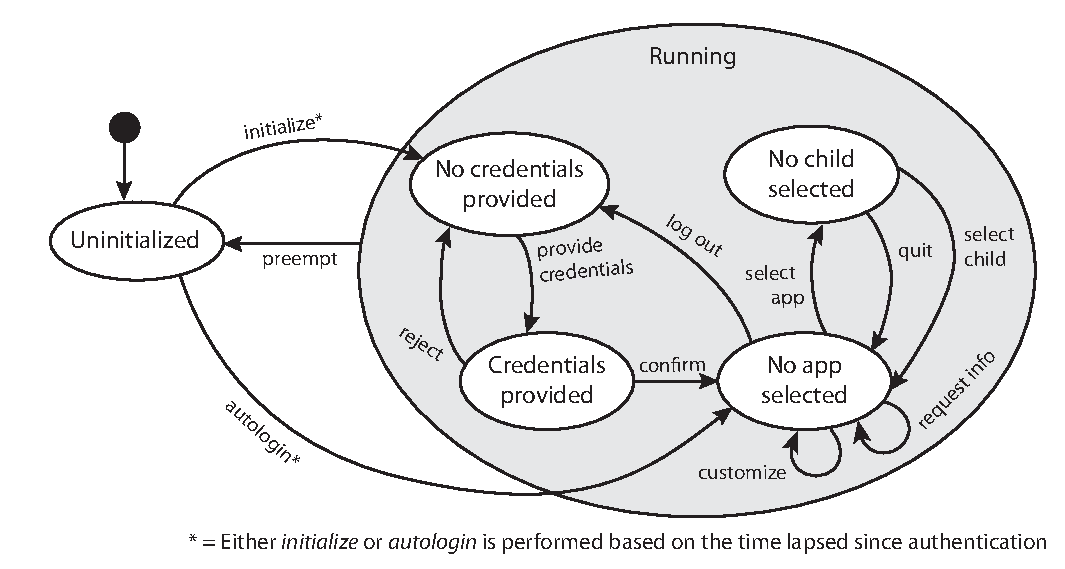
\includegraphics[width=1\textwidth]{gfx/statediagram.pdf}
	\caption{State diagram}
	\label{fig:state_diagram}
\end{figure}

\autoref{fig:state_diagram} shows all possible states and transitions, which the launcher can be in.
The ``no crendentials provided''-state is the initial state which the system is in, after initial execution.
This state, together with the ``credentials provided''-state, handles authentication and confirmation of the guardian currently using the launcher.
After confirmation, the launcher enters the ``no app selected''-state, where the launcher waits for user input, on which app to select for execution. \\

The ``no child selected''-state shows the state which the launcher is in, while waiting for user input on which child profile to use, when executing the previously selected app.
Note that the actual runtime of the selected app is not modelled here, as the launcher regardless of the selected app, transits back to the ``no app selected''-state. \\

Should the launcher be preempted by an external force, such as the OS or hardware failiure, then the launcher will enter the ``terminated''-state.
Depending on how long after authentication that the launcher is resumed after preemption, the launcher may transit to the ``no app selected''-state, instead of the ``No credentials provided''-state.
This is to take the \emph{autologin} feature -- described in \autoref{backlog:autologin} -- into account.
